

\QCMautoevaluation{Pour chaque question, plusieurs réponses sont
  proposées.  Déterminer celles qui sont correctes.}


\begin{QCM}

\begin{GroupeQCM}

\begin{exercice}Si $RKE$ est rectangle en $K$ alors...
\begin{ChoixQCM}{4}
\item $RK^2 = RE^2 + EK^2$
\item $EK^2 = ER^2 + RK^2$
\item $RE^2 = RK^2 + KE^2$
\item $KE^2 = RE^2 – RK^2$
\end{ChoixQCM}
\begin{corrige}
\reponseQCM{b}
\end{corrige}
\end{exercice}

\begin{exercice}$ABC$ est rectangle en $A$ ; $AB = 5$ et $BC = 7$ (en cm). L'arrondi au dixième de $AC$ est...
\begin{ChoixQCM}{4}
\item 8,6 cm
\item 4,8 cm
\item 4,89 cm
\item 4,9 cm
\end{ChoixQCM}
\begin{corrige}
\reponseQCM{d}
\end{corrige}
\end{exercice}

\begin{exercice}Si $KG^2 \neq KC^2 + CG^2$ alors...
\begin{ChoixQCM}{4}
\item $KCG$ n'est pas rectangle
\item $KCG$ peut être rectangle
\item $KCG$ n'est pas rectangle en $C$
\item $KCG$ est quelconque
\end{ChoixQCM}
\begin{corrige}
\reponseQCM{b c}
\end{corrige}
\end{exercice}

\begin{exercice}Si $M\in [AC]$, $N\in [BC]$ et $(MN)//(AB)$ alors...

\definecolor{zzttqq}{rgb}{0.6,0.2,0.}
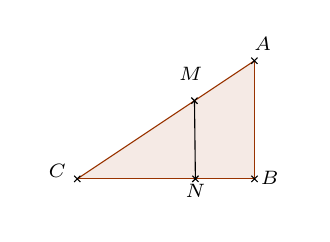
\begin{tikzpicture}[scale=0.75][line cap=round,line join=round,>=triangle 45,x=1.0cm,y=1.0cm]
\clip(1.16,0.4) rectangle (5.8,3.56);
\fill[color=zzttqq,fill=zzttqq,fill opacity=0.1] (2.,1.) -- (5.,1.) -- (5.,3.) -- cycle;
\draw [color=zzttqq] (2.,1.)-- (5.,1.);
\draw [color=zzttqq] (5.,1.)-- (5.,3.);
\draw [color=zzttqq] (5.,3.)-- (2.,1.);
\draw (4.,1.)-- (3.98461538462,2.32307692308);
\begin{scriptsize}
\draw [color=black] (2.,1.)-- ++(-1.5pt,-1.5pt) -- ++(3.0pt,3.0pt) ++(-3.0pt,0) -- ++(3.0pt,-3.0pt);
\draw[color=black] (1.66,1.14) node {$C$};
\draw [color=black] (5.,1.)-- ++(-1.5pt,-1.5pt) -- ++(3.0pt,3.0pt) ++(-3.0pt,0) -- ++(3.0pt,-3.0pt);
\draw[color=black] (5.26,1.02) node {$B$};
\draw [color=black] (5.,3.)-- ++(-1.5pt,-1.5pt) -- ++(3.0pt,3.0pt) ++(-3.0pt,0) -- ++(3.0pt,-3.0pt);
\draw[color=black] (5.14,3.28) node {$A$};
\draw [color=black] (4.,1.)-- ++(-1.5pt,-1.5pt) -- ++(3.0pt,3.0pt) ++(-3.0pt,0) -- ++(3.0pt,-3.0pt);
\draw[color=black] (4.,0.8) node {$N$};
\draw [color=black] (3.98461538462,2.32307692308)-- ++(-1.5pt,-1.5pt) -- ++(3.0pt,3.0pt) ++(-3.0pt,0) -- ++(3.0pt,-3.0pt);
\draw[color=black] (3.92,2.78) node {$M$};
\end{scriptsize}
\end{tikzpicture}
\begin{ChoixQCM}{4}
\item $\dfrac{AM}{AC}=\dfrac{BN}{BC}=\dfrac{MN}{AB}$
\item $\dfrac{CM}{CN}=\dfrac{CA}{CB}=\dfrac{MN}{AB}$
\item $\dfrac{CM}{CA}=\dfrac{CN}{CB}=\dfrac{MN}{AB}$
\item $\dfrac{CM}{CA}=\dfrac{CB}{CN}=\dfrac{MN}{AB}$
\end{ChoixQCM}
\begin{corrige}
\reponseQCM{c}
\end{corrige}
\end{exercice}

\begin{exercice}Dans le cas précédent,  $CM = 4,5$ ; $MA = 3$ et $CN = 3$ donc...
\begin{ChoixQCM}{4}
\item $CB = 2$
\item $CB = 5$
\item $BN = 2$
\item $CB = \dfrac{9}{5}$
\end{ChoixQCM}
\begin{corrige}
\reponseQCM{b}
\end{corrige}
\end{exercice}


\begin{exercice}

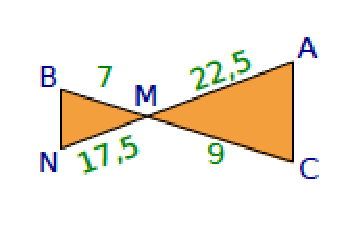
\includegraphics[scale=0.5]{T11}
\begin{ChoixQCM}{4}
\item $(AC)$ et $(BN)$ sont parallèles
\item $(AC)$ et $(BN)$ ne sont pas parallèles
\item On ne peut pas savoir si $(AC)$ 
et $(BN)$ sont parallèles
\item $\dfrac{NB}{AC}=\dfrac{MB}{MC}$
\end{ChoixQCM}
\begin{corrige}
\reponseQCM{a d}
\end{corrige}
\end{exercice}


\end{GroupeQCM}
\end{QCM}

  
